\section{Manufacturing}
\label{manufacturing}
The final stator has to be created from the cast part; the casting model is the blue outline in Figure \ref{fig:finishedmanu}. In order for the stator to reach its final redesign, a manufacturing plan must be created. All the process steps have numbers, outlined below. The premachine steps focus mainly on removing material and will complete multiple passes until an adequate amount of material is removed. Finishing, on the other hand, will only use one pass to smooth the edges of the part. The whole part will be made using a lathe \cite{lathe}. The steps and corresponding tools can be found in Table \ref{manutable} in Appendix \ref{appendixmanufacturing}. The manufacturing plan is as follows:
\begin{enumerate}
\item The first step is creating the hole in the middle of the stator. This hole will have a diameter of 30 [mm] and will be drilled through depth of the whole part.
\item Next, the top part of the stator, labeled A in Figure \ref{fig:finishedmanu}, will be machined. In this step, the level surfaces will be turned as well as pieces of the edges. In Figure \ref{fig:premachining}, the part is visualized after this premachining stage. The level surfaces of the stator are turned, but the edge is only in a preliminary stage; this is visualized using a stair step pattern along the edge.
\item After the premachining is completed, the edges in B will be finished. The edges will be smoothed out to change from the stair step pattern seen in Figure \ref{fig:premachining} to the smooth edges seen in Figure \ref{fig:finishedmanu}.
\item Next, the stator is rotated and a similar process will occur as did in Step 2. The areas labeled B in Figure \ref{fig:finishedmanu} will now be turned. Most of the material will be removed at the upper curve and the lower curve, while the flat surfaces at the lower part of B will be finished. Again, the resulting stair step pattern is visible in Figure \ref{fig:premachining}. For this turning step, the tool used will be different because we are now tooling internally rather than externally.
\item Now the edges in B will be smoothed and finished. This will result in edges like those seen in Figure \ref{fig:finishedmanu}.
\item The stator will be turned once more to machine area C. Again, the flat edges will be turned and the curve at C will be preliminarily turned.
\item Lastly, the finishing will occur for the edge in area C. 
\end{enumerate}

\begin{figure}[H]
\centering
\begin{minipage}{.5\textwidth}
  \centering
  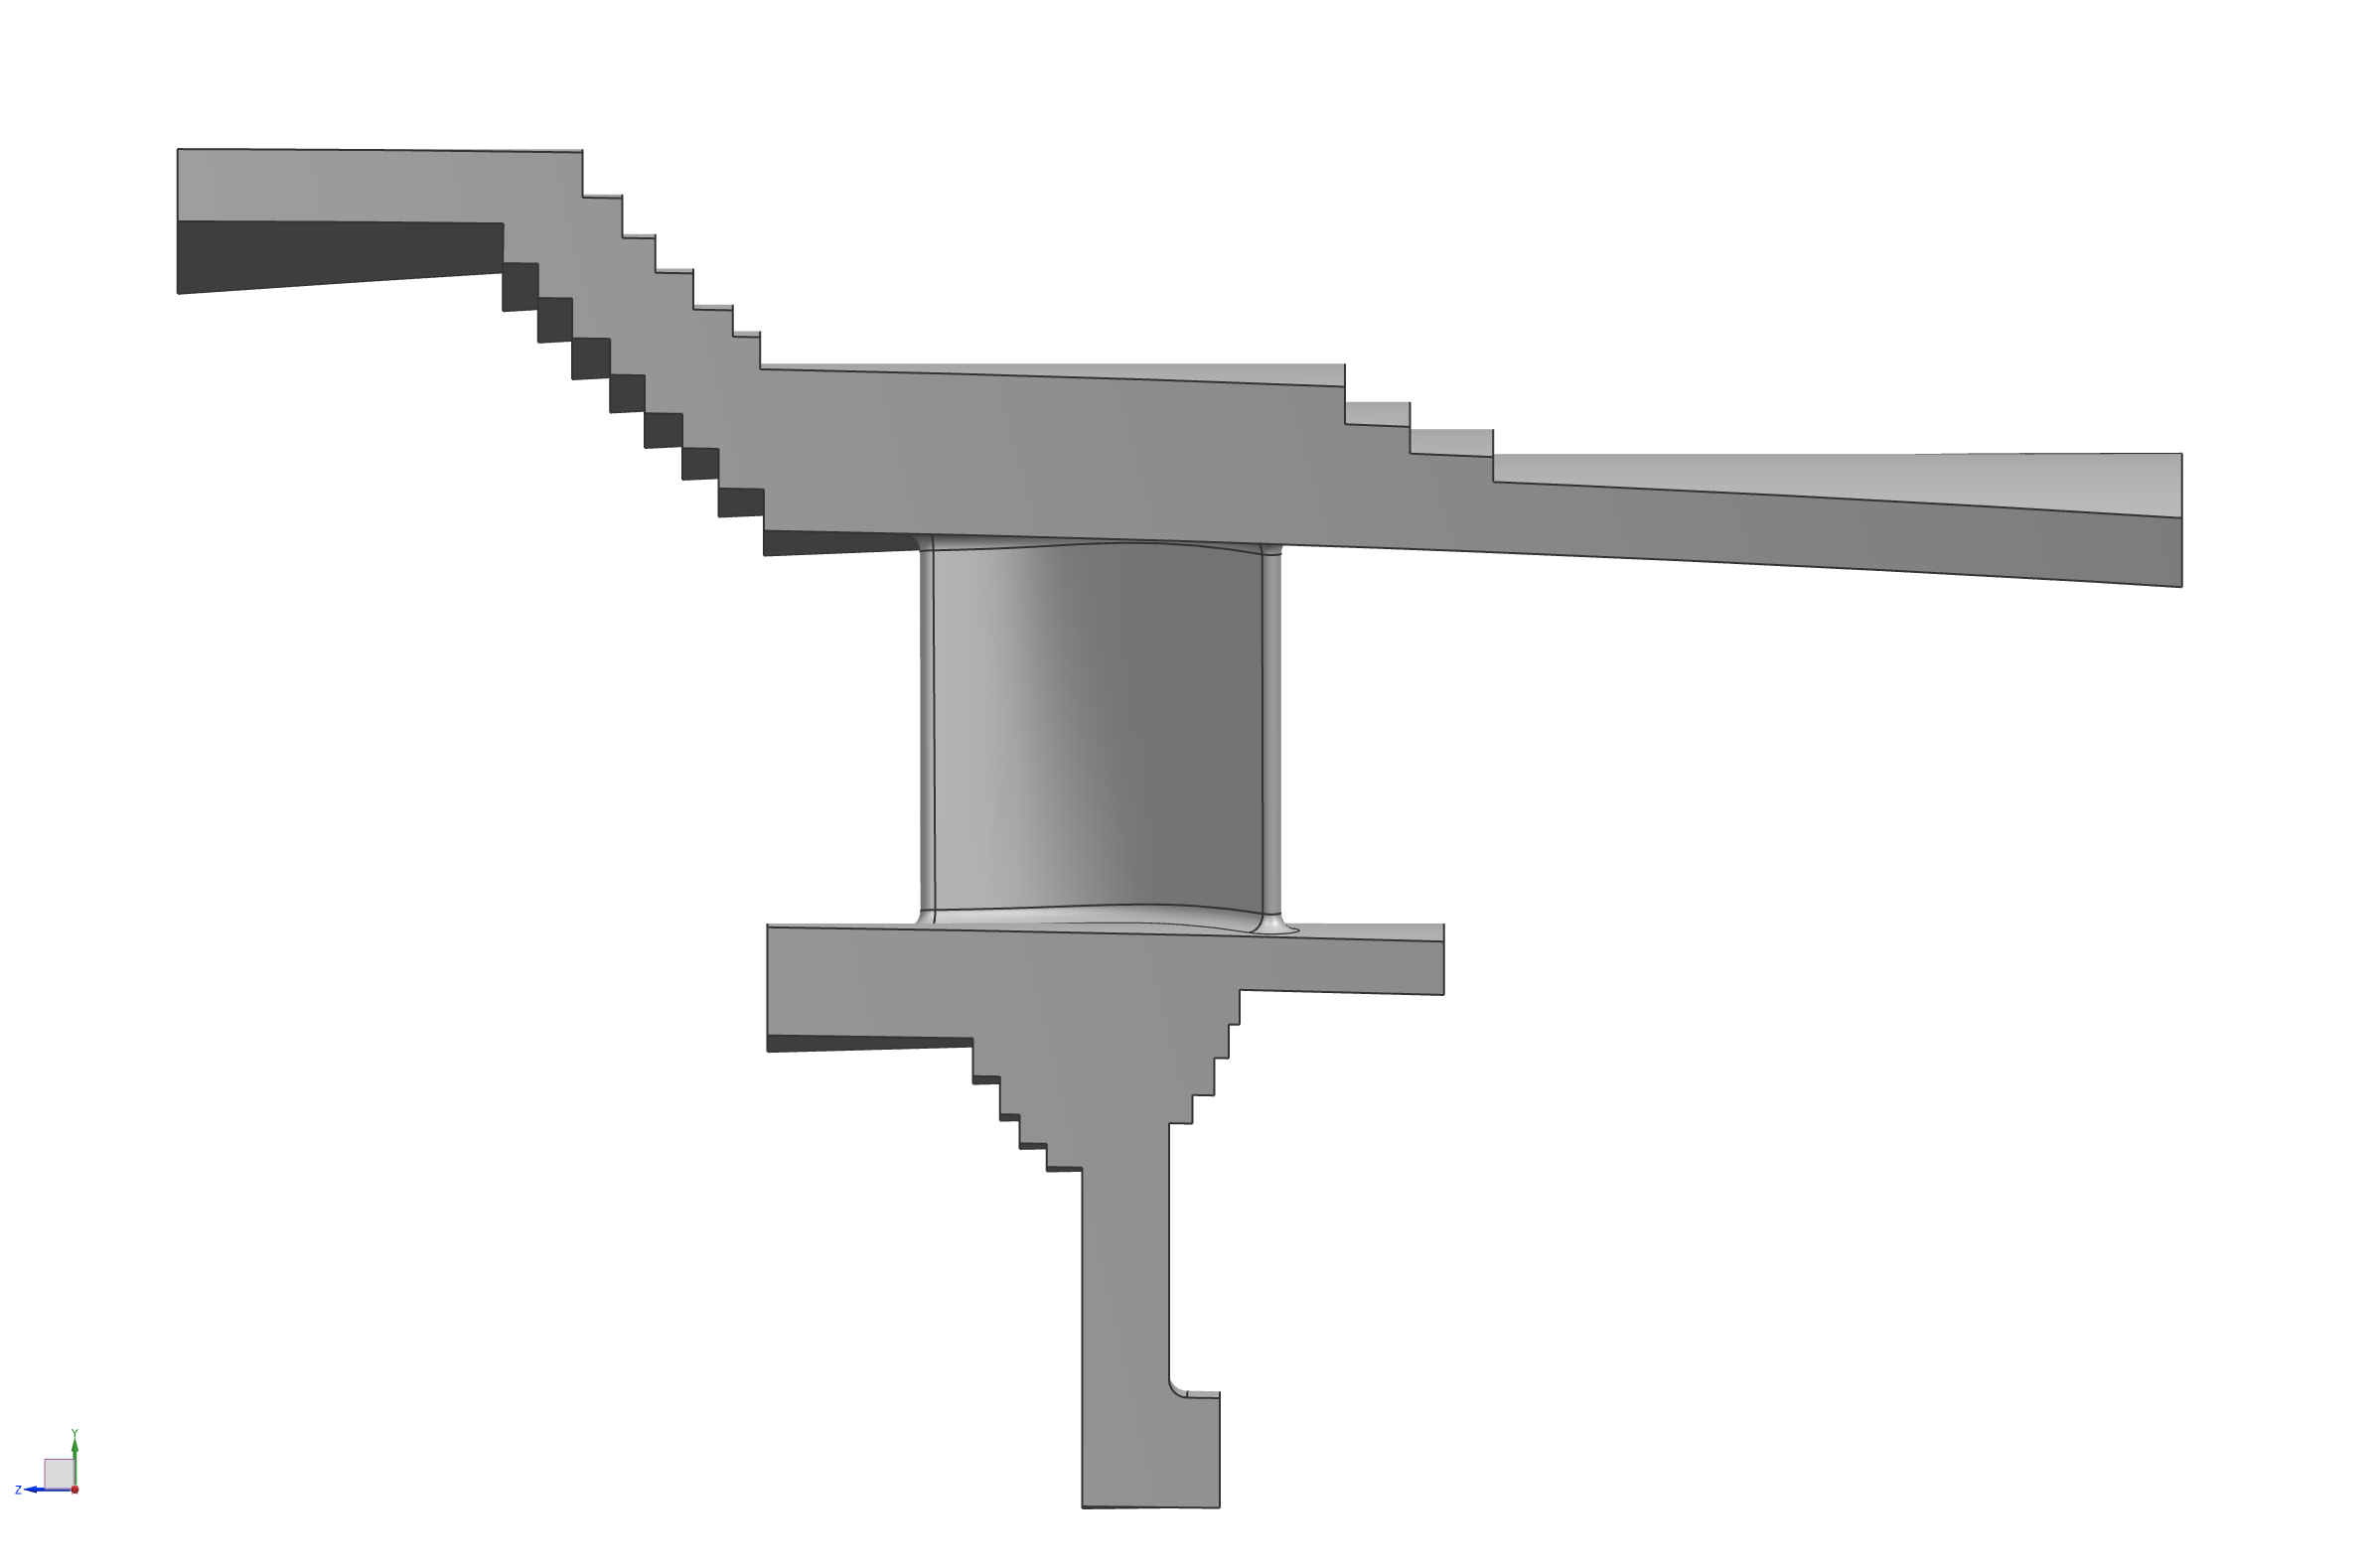
\includegraphics[width=1\linewidth]{Figures/manufacturingpart1.png}
  \captionof{figure}{Premachined Part}
  \label{fig:premachining}
\end{minipage}%
\begin{minipage}{.5\textwidth}
  \centering
  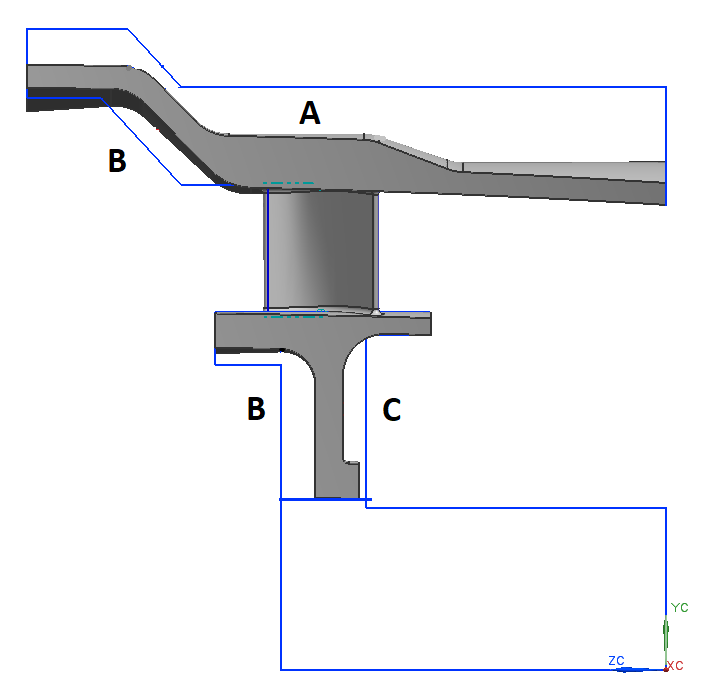
\includegraphics[width=.8\linewidth]{Figures/statormanu2.png}
  \captionof{figure}{Finished Part}
  \label{fig:finishedmanu}
\end{minipage}
\end{figure}

\newpage